%% ─────────────────────────────────────────────────────────────────────────────
%% A 9-State Markov Chain Model for Semi-Fixed Menstruation Patterns:
%% Stationary Distribution, Mean First Passage Times, and Population Heterogeneity
%%
%% Author : Dvir Ross, Shenkar College
%% Target : Mathematics (MDPI)  –  Q1 Applied Probability / Statistics
%% ─────────────────────────────────────────────────────────────────────────────
\documentclass[12pt,a4paper]{article}

%% ── Packages ─────────────────────────────────────────────────────────────────
\usepackage[margin=2.5cm]{geometry}
\usepackage{amsmath,amssymb,amsthm}
\usepackage{booktabs}
\usepackage{multirow}
\usepackage{array}
\usepackage{graphicx}
\usepackage{subcaption}
\usepackage{xcolor}
\usepackage[colorlinks=true,linkcolor=blue!60!black,
            citecolor=blue!60!black,urlcolor=blue!60!black]{hyperref}
\usepackage{natbib}
\usepackage{setspace}
\usepackage{microtype}
\usepackage{enumerate}
\usepackage{algorithm}
\usepackage{algpseudocode}
\usepackage{tikz}
\usetikzlibrary{arrows.meta,positioning,shapes.geometric,calc}
\usepackage{pgfplots}
\pgfplotsset{compat=1.18}

\onehalfspacing

%% ── Theorem environments ─────────────────────────────────────────────────────
\newtheorem{definition}{Definition}
\newtheorem{theorem}{Theorem}
\newtheorem{proposition}{Proposition}
\newtheorem{corollary}{Corollary}
\newtheorem{lemma}{Lemma}
\newtheorem{remark}{Remark}

%% ── Custom commands ──────────────────────────────────────────────────────────
\newcommand{\piv}{\boldsymbol{\pi}}
\newcommand{\mat}[1]{\mathbf{#1}}
\newcommand{\R}{\mathbb{R}}
\newcommand{\E}{\mathbb{E}}
\newcommand{\haflaga}{\textit{Haflaga}}
\newcommand{\dilug}{\textit{Dilug}}
\newcommand{\veset}{\textit{veset}}

%% ─────────────────────────────────────────────────────────────────────────────
\begin{document}

%% ── Title block ──────────────────────────────────────────────────────────────
\title{\textbf{A 9-State Markov Chain Model for Semi-Fixed Menstruation Patterns:
Stationary Distribution, Mean First Passage Times, and Population Heterogeneity}}

\author{%
  Dvir Ross\\[4pt]
  \small Department of Software Engineering and Computer Science,\\
  \small Shenkar College of Engineering, Design and Art,\\
  \small Ramat Gan, Israel\\[2pt]
  \small \texttt{dvirross@shenkar.ac.il}
}

\date{}
\maketitle

%% ── Abstract ─────────────────────────────────────────────────────────────────
\begin{abstract}
\noindent
We introduce and analyse a nine-state, discrete-time, homogeneous Markov chain
that models the longitudinal dynamics of \emph{semi-fixed menstruation}
(\textit{veset hatzi kavu'a}), a central construct of Jewish Halachic law governing
anticipatory pre-menstrual abstinence. The state space encodes both the ordinal
position of a cycle within a semi-fixed stretch and the sub-type of the accumulated
cycle-length range: short ($r_{\max} < 29$), normal ($29 \le r_{\min}$ or
$r_{\max} \le 31$), or long ($r_{\min} > 31$), yielding nine states whose
transition structure is fully determined by the Halachic definition---independent
of data.

We prove that the $9\times9$ transition matrix has an exact $3\times3$ block
structure that reduces the stationary computation to a $3\times3$ eigenproblem,
provide a closed-form block formula for the stationary distribution $\piv$, and
establish irreducibility and aperiodicity.  Using a Natural Family Planning (NFP)
dataset of 1{,}221 cycles from 98 participants (after excluding
\haflaga-established clients), we estimate $\hat{\mat{P}}$ and obtain:
$\pi_{S_{32}} \approx 54.2\%$ (normal semi-fixed, full Halachic obligations),
$\pi_{S_{31}}+\pi_{S_{33}} \approx 8.9\%$ (favourable semi-fixed, no extra
obligations), with 95\% bootstrap confidence intervals of
$[48.8\%, 59.1\%]$ and $[6.1\%, 12.1\%]$, respectively.  The spectral gap
$\delta = 1 - |\lambda_2| \approx 0.297$ implies the chain reaches stationarity
within $\le 23$ cycles, validated by a Chapman-Kolmogorov test
($p = 0.97$, confirming the order-1 Markov assumption).

We compute mean first passage times (MFPTs) to the favourable set
$\{S_{31},S_{33}\}$ from every state: a woman starting fresh (state $S_{11}$)
expects to reach a favourable state in $17.9$ cycles on average.  Stratifying the
sample into three sub-populations by attained semi-fixed sub-type reveals
significant heterogeneity (Kruskal-Wallis $H = 386.0$, $p < 10^{-84}$): for
short-cycle women ($G_{31}$, mean $\tilde{L}\approx27.6$~days) the group-specific
sub-chain yields $\pi^{(31)}_{S_{31}} \approx 18.6\%$ and an MFPT of only
$4.7$ cycles, while $G_{32}$ (normal-cycle) women effectively never reach a
favourable state.  A threshold sensitivity analysis over $\pm2$-day perturbations
shows that the all-semi-fixed probability ($63.1\%$) is stable across all
configurations, while the favourable probability ranges from $2.8\%$ to $12.1\%$.

\medskip
\noindent\textbf{Keywords:} Markov chain; stationary distribution; mean first
passage time; spectral gap; semi-fixed menstruation; Halachic law; natural
family planning; population heterogeneity; applied probability
\end{abstract}

\newpage

%% ─────────────────────────────────────────────────────────────────────────────
\section{Introduction}
\label{sec:intro}
%% ─────────────────────────────────────────────────────────────────────────────

The menstrual cycle is governed by the hypothalamic-pituitary-ovarian axis and
exhibits substantial variability both within and across individuals
\citep{Treloar1967, Chiazze1968, Munster1992}.  Understanding this variability
has broad applications: reproductive medicine uses cycle statistics for infertility
diagnostics; natural family planning (NFP) methods convert cycle-length observations
into fertility estimates \citep{Fehring2006}; and mobile apps have demonstrated
feasibility of population-scale tracking \citep{Symul2019, Bull2019}.

In Jewish Halachic law, the laws of \textit{Nidah} define obligatory spousal
separation following menstruation and govern the anticipation of the next onset.
A woman is required to observe pre-menstrual abstinence on the day she anticipates
her next cycle will begin.  The extent of this obligation depends critically on
whether and what type of \emph{fixed} or \emph{semi-fixed} menstruation pattern she
has established.  Quantitative analysis of these patterns from a probability and
statistics viewpoint is still nascent: \citet{Ross2023stat} analysed the
statistical properties of abstinence obligations; \citet{Ross2024reliability}
studied reporting reliability in survey data; and \citet{Ross2024markov} modelled
\haflaga{} fixed menstruation as a two-state Markov chain.

A woman establishes \emph{semi-fixed menstruation} (\textit{veset hatzi kavu'a})
when two consecutive cycle lengths fall within a shared interval; she remains
semi-fixed as long as each subsequent length stays within that interval.  Despite
being the modal long-run regime (as our analysis confirms), semi-fixed menstruation
has received no prior probabilistic treatment.  Its Halachic implications depend
not only on the onset of the semi-fixed state but also on the sub-type of the
accumulated cycle-length range, which determines whether the daily obligations at
day~30 and at the monthly Halachic date are binding.

\subsection*{Contributions}

This paper makes the following contributions:

\begin{enumerate}
  \item \textbf{Block-structured Markov chain.}  We define a nine-state
        Markov chain whose transition structure is a direct algebraic consequence
        of the Halachic definition, and prove an exact $3\times3$ block
        decomposition (Theorem~\ref{thm:block}), reducing the $9\times9$
        stationary eigenproblem to a $3\times3$ one (Proposition~\ref{prop:formula}).

  \item \textbf{Stationary distribution with uncertainty quantification.}
        We derive $\piv$ analytically and provide 95\% bootstrap confidence
        intervals ($B = 2{,}000$ bootstrap replications over clients) on all nine
        state probabilities and their aggregates.

  \item \textbf{Validation of the Markov property.}  We confirm that the
        order-1 Markov assumption is adequate at the two-step horizon via a
        Chapman-Kolmogorov test ($\chi^2 = 19.0$, $p = 0.97$).

  \item \textbf{Spectral gap and mixing time.}  We compute the spectral gap
        $\delta = 0.297$ and establish an upper bound of 23 cycles on the
        $\varepsilon$-mixing time for $\varepsilon = 0.01$.

  \item \textbf{Mean first passage times.}  We compute and interpret the MFPT
        from every state to the favourable set $\{S_{31}, S_{33}\}$, providing
        a practically interpretable quantity: the expected wait until a woman is
        free of the additional Halachic obligations.

  \item \textbf{Threshold sensitivity and sub-population analysis.}
        We show that the all-semi-fixed probability is robust to $\pm2$-day
        threshold perturbations, while group-specific sub-chains reveal that the
        population-average MFPT substantially overestimates the wait for
        short-cycle women.
\end{enumerate}

\subsection*{Paper organisation}

Section~\ref{sec:background} introduces the Halachic framework and mathematical
background (Markov chains, spectral theory, first passage times).
Section~\ref{sec:data} describes the dataset and pre-processing.
Section~\ref{sec:model} defines the chain, proves its block structure, and derives
the analytical formula for $\piv$.
Section~\ref{sec:results} presents all empirical results.
Section~\ref{sec:discussion} discusses implications and limitations.
Section~\ref{sec:conclusion} concludes.

%% ─────────────────────────────────────────────────────────────────────────────
\section{Background}
\label{sec:background}
%% ─────────────────────────────────────────────────────────────────────────────

\subsection{Halachic Framework}
\label{sec:halacha}

The Halachic interval between two consecutive menstrual onsets equals the calendar
cycle length \emph{plus one}, because Halachic law counts the day of onset as the
first day of the new cycle rather than the last day of the preceding one
\citep{ShulchanAruch}.  If the calendar length is $L$~days, the Halachic
\emph{haflaga} is $\tilde{L} = L + 1$.  All analyses use $\tilde{L}$.

\begin{definition}[Semi-fixed menstruation]\label{def:semi-fixed}
A woman establishes \emph{semi-fixed menstruation} when two consecutive Halachic
cycle lengths $\tilde{L}_{n-1}$ and $\tilde{L}_{n}$ satisfy
$r_{\min} := \min(\tilde{L}_{n-1},\tilde{L}_{n})$ and
$r_{\max} := \max(\tilde{L}_{n-1},\tilde{L}_{n})$.
Her \emph{semi-fixed interval} is $[r_{\min}, r_{\max}]$.
She remains semi-fixed while each subsequent length $\tilde{L}_{n+k}$ satisfies
$r_{\min} \le \tilde{L}_{n+k} \le r_{\max}$; the interval can only widen.
A length outside the interval dissolves the pattern and resets the process.
\end{definition}

The Halachic obligations triggered by a semi-fixed state depend on whether the
anticipated day (day~30 from the last onset) and the monthly Halachic date fall
within the semi-fixed interval \citep{NishmatAvraham}:
\begin{itemize}
  \item \textbf{Short range} ($r_{\max} < 29$): both day~30 and the monthly
        date fall above the interval; \emph{no additional abstinence required}.
  \item \textbf{Normal range} ($r_{\min} \le 31$ and $r_{\max} \ge 29$):
        at least one of the two obligation days falls within the interval;
        full anticipatory abstinence required.
  \item \textbf{Long range} ($r_{\min} > 31$): day~30 falls below the interval;
        the monthly-date obligation depends on the specific date.
        In the model we treat long-range as the second \emph{favourable} sub-type,
        consistent with Halachic practice in most communities \citep{NishmatAvraham}.
\end{itemize}

\subsection{Markov Chains: Stationarity, Spectral Theory, and First Passage Times}
\label{sec:mc-background}

A \emph{discrete-time finite Markov chain} is a stochastic process
$\{X_n\}_{n \ge 1}$ over a finite state space $\mathcal{S}$ with homogeneous
transition kernel $p_{ij} = \Pr(X_{n+1}=j \mid X_n=i)$ and matrix
$\mat{P} = (p_{ij})$ \citep{Norris1997}.

\paragraph{Stationary distribution.}
If the chain is irreducible and aperiodic it possesses a unique stationary
distribution $\piv$ satisfying $\piv\mat{P} = \piv$, $\mathbf{1}^\top\piv = 1$,
$\pi_k > 0$ for all $k$ \citep{KemenySnell1960}. Equivalently,
\begin{equation}\label{eq:stationary}
  \mat{P}^\top\piv = \piv, \qquad \|\piv\|_1 = 1,
\end{equation}
so $\piv$ is the eigenvector of $\mat{P}^\top$ for eigenvalue~1.

\paragraph{Spectral gap and mixing time.}
Denote the eigenvalues of $\mat{P}$ by $1 = \lambda_1 \ge |\lambda_2| \ge \cdots$
For an irreducible aperiodic chain, $|\lambda_2| < 1$, and the
\emph{spectral gap} $\delta := 1 - |\lambda_2|$ governs the rate of convergence
to stationarity.  Concretely, the total variation distance after $t$ steps
satisfies $\|P^t(x,\cdot) - \piv\|_{\rm TV} \le C\,(1-\delta)^t$ \citep{Bremaud1999}.
A standard mixing-time bound is
\begin{equation}\label{eq:mixing}
  t_{\rm mix}(\varepsilon) \le \frac{1}{\delta}\ln\!\left(\frac{K}{\varepsilon}\right),
\end{equation}
where $K = |\mathcal{S}|$ \citep{Norris1997}.

\paragraph{Mean first passage times.}
For target state $j$ or target set $F \subseteq \mathcal{S}$, the \emph{mean first
passage time} (MFPT) from state $i$ is
$m_{iF} = \E[\tau_F \mid X_0 = i]$, where $\tau_F = \min\{n \ge 1 : X_n \in F\}$.
The MFPT vector $\mathbf{m}_F = (m_{iF})_{i \notin F}$ solves the linear system
\begin{equation}\label{eq:mfpt}
  \mathbf{m}_F = \mathbf{1} + \mat{P}_{-F}\,\mathbf{m}_F,
  \quad\text{i.e.,}\quad
  (\mat{I} - \mat{P}_{-F})\,\mathbf{m}_F = \mathbf{1},
\end{equation}
where $\mat{P}_{-F}$ is $\mat{P}$ restricted to states outside $F$ \citep{KemenySnell1960}.
The mean \emph{return} time to state $j$ is $1/\pi_j$.

\subsection{Related Work}
\label{sec:related}

Longitudinal modelling of menstrual cycles has largely focused on either
population-level distributional characterisation
\citep{Treloar1967, Chiazze1968, Guo2006, Symul2019, Bull2019}
or sequential cycle-length prediction \citep{Liao2018}.
Markov chain approaches to reproductive cycles are relatively recent:
\citet{Colombo2000} modelled daily fecundability as a Markov process, and
\citet{Pierson2001} used Markov-type state transitions to describe
peri-ovulatory endometrial changes.

Within the Halachic domain, \citet{Ross2024markov} introduced a Markov chain
for \haflaga{} fixed menstruation (a simpler two-level system), and
\citet{Ross2023stat} applied statistical hypothesis testing to abstinence-pattern
frequencies.  The present paper extends this line of work to the
substantially richer nine-state semi-fixed system, adding spectral analysis,
MFPTs, bootstrap uncertainty quantification, and a block-structure theorem
that are absent from prior work.

%% ─────────────────────────────────────────────────────────────────────────────
\section{Data and Pre-processing}
\label{sec:data}
%% ─────────────────────────────────────────────────────────────────────────────

\subsection{Dataset}

We use an anonymised NFP dataset collected by certified instructors.  Each record
is one menstrual cycle for one participant and includes the calendar cycle length,
cycle number within the observation window, and demographic covariates (age, BMI,
parity, and others). The raw data contain 1{,}665 records from 133 clients.

\subsection{Pre-processing}

After removing duplicate \texttt{(ClientID, CycleNumber)} pairs and nine anomalous
records (client 8107, cycles 45--53, identified during data collection) and
restricting to participants with at least five recorded cycles, the \emph{cleaned}
dataset comprises \textbf{1{,}554 cycles from 118 clients} (mean 13.2 cycles;
median 12; range 5--45).

\subsection{Halachic Cycle Length and Descriptive Statistics}

All analyses use $\tilde{L} = L + 1$ (Definition~\ref{def:semi-fixed}).
Table~\ref{tab:descriptives} reports descriptive statistics.

\begin{table}[ht]
\centering
\caption{Descriptive statistics of $\tilde{L}$ in the cleaned dataset
  ($n = 1{,}554$ cycles, 118 clients).}
\label{tab:descriptives}
\begin{tabular}{lc}
\toprule
\textbf{Statistic} & \textbf{Value} \\
\midrule
Cycles / Clients & 1{,}554 / 118 \\
Mean (SD)   & 30.27 (3.86) days \\
Median (IQR)& 29.50 (28--32) days \\
Min -- Max  & 19 -- 55 days \\
Skewness    & 1.38 \\
Excess kurtosis & 5.71 \\
Shapiro-Wilk $W$ & 0.924 ($p < 10^{-30}$) \\
\bottomrule
\end{tabular}
\end{table}

The right-skewed, leptokurtic distribution is consistent with
\citet{Guo2006} and \citet{Bull2019}.  Non-normality motivates non-parametric
inference throughout.

\subsection{Exclusion of \haflaga-Fixed Participants}
\label{sec:exclusion}

Participants who established a \haflaga{} fixed menstruation (three consecutive
equal Halachic cycle lengths) operate under a distinct Halachic regime whose
Markov dynamics were studied by \citet{Ross2024markov}.  Including them would
introduce structural autocorrelations incompatible with the semi-fixed model.
We exclude the 20 such participants, yielding the
\textbf{analysis dataset of 1{,}221 cycles from 98 clients}.

%% ─────────────────────────────────────────────────────────────────────────────
\section{The 9-State Markov Chain: Definition and Theory}
\label{sec:model}
%% ─────────────────────────────────────────────────────────────────────────────

\subsection{State Space}
\label{sec:states}

\begin{definition}[State space $\mathcal{S}$]\label{def:states}
Nine states $\mathcal{S} = \{S_{11}, S_{12}, S_{13},
S_{21}, S_{22}, S_{23}, S_{31}, S_{32}, S_{33}\}$ are defined, where the
\emph{first index} encodes the ordinal position within the current stretch and
the \emph{second index} encodes the range sub-type:
\begin{align*}
\text{First index:}\quad
  &1 \Rightarrow \text{first cycle of a new stretch},\\
  &2 \Rightarrow \text{second cycle (interval being formed)},\\
  &3 \Rightarrow \text{third or later cycle (semi-fixed achieved)}.\\[4pt]
\text{Second index:}\quad
  &1 \Rightarrow r_{\max} < 29 \quad (\text{short range, favourable}),\\
  &2 \Rightarrow 29 \le r_{\min} \text{ or } r_{\max} \le 31
                 \quad (\text{normal range, obligations}),\\
  &3 \Rightarrow r_{\min} > 31 \quad (\text{long range, favourable}).
\end{align*}
\end{definition}

The \emph{semi-fixed states} are $S_{3\bullet} = \{S_{31}, S_{32}, S_{33}\}$;
among them, $S_{31}$ and $S_{33}$ are the \emph{favourable} states requiring
no additional abstinence obligations.

\subsection{State Assignment Algorithm}
\label{sec:algorithm}

Algorithm~\ref{alg:state} assigns states sequentially to cycle lengths for a
single participant.

\begin{algorithm}[ht]
\caption{Semi-fixed state assignment (single participant)}
\label{alg:state}
\begin{algorithmic}[1]
\Require Sequence $(\tilde{L}_1,\ldots,\tilde{L}_N)$,
         thresholds $\theta_s = 29$, $\theta_\ell = 31$
\Ensure State sequence $(X_1,\ldots,X_N)$
\State $r_{\min} \gets \tilde{L}_1$;\; $r_{\max} \gets \tilde{L}_1$;\;
       $\text{sf} \gets 0$ \Comment{$\text{sf}=1$: currently semi-fixed}
\State $X_1 \gets \textsc{Sub}(r_{\min}, r_{\max}, \text{``S1''})$
\For{$i = 2, \ldots, N$}
  \If{$\text{sf}=1$ \textbf{and} $(\tilde{L}_i < r_{\min}$ \textbf{or}
      $\tilde{L}_i > r_{\max})$}
    \State $r_{\min}\!\gets\!\tilde{L}_i$;\; $r_{\max}\!\gets\!\tilde{L}_i$;\;
           $\text{sf}\!\gets\!0$;\;
           $X_i \gets \textsc{Sub}(r_{\min}, r_{\max}, \text{``S1''})$
  \ElsIf{$\text{sf}=0$ \textbf{and} $X_{i-1}$ starts with ``S1''}
    \State $r_{\min}\!\gets\!\min(r_{\min},\tilde{L}_i)$;\;
           $r_{\max}\!\gets\!\max(r_{\max},\tilde{L}_i)$;\;
           $X_i \gets \textsc{Sub}(r_{\min}, r_{\max}, \text{``S2''})$
  \Else
    \State $r_{\min}\!\gets\!\min(r_{\min},\tilde{L}_i)$;\;
           $r_{\max}\!\gets\!\max(r_{\max},\tilde{L}_i)$;\;
           $\text{sf}\!\gets\!1$;\;
           $X_i \gets \textsc{Sub}(r_{\min}, r_{\max}, \text{``S3''})$
  \EndIf
\EndFor
\Procedure{Sub}{$r_{\min}, r_{\max}, \text{prefix}$}
  \If{$r_{\max} < \theta_s$} \Return prefix$+$``1''
  \ElsIf{$r_{\min} > \theta_\ell$} \Return prefix$+$``3''
  \Else\ \Return prefix$+$``2''
  \EndIf
\EndProcedure
\end{algorithmic}
\end{algorithm}

\begin{remark}\label{rem:monotone}
Within any stretch, the range $[r_{\min}, r_{\max}]$ is monotonically
non-decreasing in width.  Consequently, the sub-type index can only
transition $1 \to 2$ or $2 \to 3$ within a stretch---it never decreases.
This is a direct algebraic consequence of the Halachic rule that the interval
can only widen.
\end{remark}

\subsection{Block Structure of the Transition Matrix}
\label{sec:block}

Partition the nine states into three levels $L_1 = \{S_{1\bullet}\}$,
$L_2 = \{S_{2\bullet}\}$, $L_3 = \{S_{3\bullet}\}$ (each of size three).
Write the transition matrix in $3 \times 3$ block form:
\begin{equation}\label{eq:block}
  \mat{P} =
  \begin{pmatrix}
    \mat{0} & \mat{A} & \mat{0} \\
    \mat{0} & \mat{0} & \mat{B} \\
    \mat{C} & \mat{0} & \mat{D}
  \end{pmatrix},
\end{equation}
where $\mat{A} \in \mathbb{R}^{3\times3}$ is the $L_1 \to L_2$ block,
$\mat{B} \in \mathbb{R}^{3\times3}$ is $L_2 \to L_3$,
$\mat{C} \in \mathbb{R}^{3\times3}$ is $L_3 \to L_1$, and
$\mat{D} \in \mathbb{R}^{3\times3}$ is $L_3 \to L_3$ (diagonal self-loops).

\begin{theorem}[Block structure]\label{thm:block}
For any realization of the semi-fixed menstruation process:
\begin{enumerate}[(i)]
  \item $L_1$-states transition only to $L_2$-states (block $\mat{A}$).
  \item $L_2$-states transition only to $L_3$-states (block $\mat{B}$).
  \item $L_3$-states transition either to $L_1$-states (block $\mat{C}$)
        or self-loop within $L_3$ (block $\mat{D}$).
  \item The off-diagonal blocks $\mat{P}_{L_1,L_3}$,
        $\mat{P}_{L_2,L_1}$, $\mat{P}_{L_2,L_2}$, $\mat{P}_{L_3,L_2}$
        are identically zero.
\end{enumerate}
\end{theorem}

\begin{proof}
(i) After a reset (entering $L_1$), the next cycle forms the second consecutive
cycle, placing the chain in $L_2$ by definition.  A transition from $L_1$ to
$L_1$ would require two resets in a row, which is impossible since an $L_1$-cycle
is always succeeded by its pair.  Transition to $L_3$ would skip the
two-cycle acquisition requirement, violating the definition.

(ii) The second cycle in a stretch advances the chain to $L_3$ (semi-fixed
established).  Return to $L_1$ would require a break, but a break resets the
range to a single value, yielding $L_1$, not $L_2$.  Self-loop within $L_2$
is impossible since each $L_2$-cycle is the \emph{second} in a stretch, and the
third cycle either continues (entering $L_3$) or breaks (entering $L_1$).

(iii) An $L_3$-cycle either continues semi-fixed (self-loop within $L_3$, possibly
changing sub-type due to range widening) or is broken by the new cycle length
falling outside the range, resetting to $L_1$.  Transition from $L_3$ to $L_2$
would require being simultaneously the second cycle of a new stretch and already
semi-fixed, a contradiction.
\end{proof}

\begin{proposition}[Analytical formula for $\piv$]\label{prop:formula}
Under the block structure~\eqref{eq:block}, the stationary distribution satisfies:
\begin{align}
  \piv_{L_1} &= \text{(left eigenvector of }\mat{M}\text{ for eigenvalue 1)},
              \label{eq:piL1}\\
  \piv_{L_2} &= \piv_{L_1}\mat{A},
              \label{eq:piL2}\\
  \piv_{L_3} &= \piv_{L_1}\mat{A}\mat{B}(\mat{I}-\mat{D})^{-1},
              \label{eq:piL3}
\end{align}
where $\mat{M} = \mat{A}\mat{B}(\mat{I}-\mat{D})^{-1}\mat{C}$.
The full vector $\piv$ is obtained by concatenating $\piv_{L_1}$, $\piv_{L_2}$,
$\piv_{L_3}$ and normalising.
\end{proposition}

\begin{proof}
The stationarity equations $\piv\mat{P} = \piv$ decompose under~\eqref{eq:block} as:
\begin{align*}
  \piv_{L_1} &= \piv_{L_3}\mat{C},                      \tag{S1}\\
  \piv_{L_2} &= \piv_{L_1}\mat{A},                      \tag{S2}\\
  \piv_{L_3} &= \piv_{L_2}\mat{B} + \piv_{L_3}\mat{D}.  \tag{S3}
\end{align*}
From (S3): $\piv_{L_3}(\mat{I}-\mat{D}) = \piv_{L_2}\mat{B}$, so
$\piv_{L_3} = \piv_{L_2}\mat{B}(\mat{I}-\mat{D})^{-1}$ (since $\mat{D}$ is
diagonal with eigenvalues in $(0,1)$, so $\mat{I}-\mat{D}$ is invertible).
Substituting (S2): $\piv_{L_3} = \piv_{L_1}\mat{A}\mat{B}(\mat{I}-\mat{D})^{-1}$.
Inserting into (S1): $\piv_{L_1} = \piv_{L_1}\mat{M}$, i.e., $\piv_{L_1}$ is
the left eigenvector of $\mat{M}$ for eigenvalue 1.  Since $\mat{M}$ is
$3\times3$, this is a rank-reduced eigenproblem.  Normalisation gives $\piv$.
\end{proof}

This proposition reduces the $9\times9$ eigenproblem to a $3\times3$ one,
and provides a transparent closed-form expression for $\piv$ in terms of the
four submatrices $\mat{A}$, $\mat{B}$, $\mat{C}$, $\mat{D}$.

\subsection{Irreducibility and Aperiodicity}
\label{sec:irred}

\begin{proposition}\label{prop:stationary}
The Markov chain with any empirically estimated $\hat{\mat{P}}$ satisfying
the block structure~\eqref{eq:block} (with $\mat{A}$, $\mat{B}$, $\mat{C}$,
$\mat{D}$ all having full row-support) is irreducible and aperiodic, hence
admits a unique stationary distribution $\piv$.
\end{proposition}

\begin{proof}[Sketch]
\emph{Irreducibility.}  From any $S_{1k}$ state, the path
$S_{1k} \to S_{2k} \to S_{3k} \to S_{1k'}$ has positive probability by the
block structure.  From any $S_{3k}$ state, a path back through $L_1 \to L_2 \to L_3$
also has positive probability.  Thus all states communicate within at most four
steps.

\emph{Aperiodicity.}  States in $L_3$ have positive self-loop probabilities
(diagonal of $\mat{D}$ is positive), so their period is 1.  Since all states
communicate, the entire chain has period 1.
\end{proof}

\subsection{State Diagram}
\label{sec:diagram}

Figure~\ref{fig:state-diagram} illustrates the directed transition graph with
estimated probabilities.  The block structure is immediately apparent: $L_1$
and $L_2$ form a deterministic pipeline, while $L_3$ states either persist
(high self-loop) or reset the process.

\begin{figure}[ht]
\centering
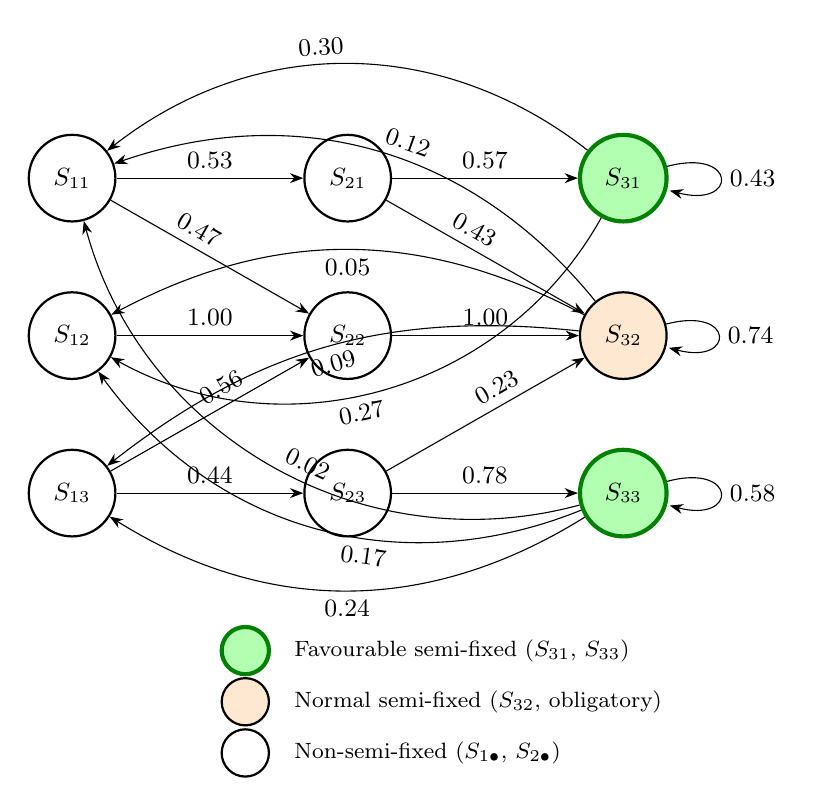
\begin{tikzpicture}[
  every node/.style={font=\small},
  state/.style={draw, circle, minimum size=1.1cm, thick, fill=white},
  sfstate/.style={draw, circle, minimum size=1.1cm, thick, fill=orange!18},
  favstate/.style={draw, circle, minimum size=1.1cm, thick, fill=green!30,
                   line width=1.5pt, draw=green!50!black},
  bend angle=18,
  auto,
  >=Stealth
]

\node[state]   (S11) at (0,4)    {$S_{11}$};
\node[state]   (S12) at (0,2)    {$S_{12}$};
\node[state]   (S13) at (0,0)    {$S_{13}$};

\node[state]   (S21) at (3.5,4)  {$S_{21}$};
\node[state]   (S22) at (3.5,2)  {$S_{22}$};
\node[state]   (S23) at (3.5,0)  {$S_{23}$};

\node[favstate](S31) at (7,4)    {$S_{31}$};
\node[sfstate] (S32) at (7,2)    {$S_{32}$};
\node[favstate](S33) at (7,0)    {$S_{33}$};

\draw[->] (S11) -- node[above,sloped]{$0.53$} (S21);
\draw[->] (S11) -- node[above,sloped,pos=0.4]{$0.47$} (S22);
\draw[->] (S12) -- node[above]{$1.00$} (S22);
\draw[->] (S13) -- node[above,sloped,pos=0.6]{$0.56$} (S22);
\draw[->] (S13) -- node[above,sloped]{$0.44$} (S23);

\draw[->] (S21) -- node[above]{$0.57$} (S31);
\draw[->] (S21) -- node[above,sloped,pos=0.4]{$0.43$} (S32);
\draw[->] (S22) -- node[above]{$1.00$} (S32);
\draw[->] (S23) -- node[above,sloped,pos=0.6]{$0.23$} (S32);
\draw[->] (S23) -- node[above]{$0.78$} (S33);

\draw[->, bend right=38] (S31) edge node[above,sloped,pos=0.55]{$0.30$} (S11);
\draw[->, bend left=45]  (S31) edge node[below,sloped,pos=0.55]{$0.27$} (S12);
\draw[->, bend right=35] (S32) edge node[above,sloped,pos=0.45]{$0.12$} (S11);
\draw[->, bend right=28] (S32) edge node[below,sloped]{$0.05$} (S12);
\draw[->, bend right=22] (S32) edge node[below,sloped]{$0.09$} (S13);
\draw[->, bend left=45]  (S33) edge node[above,sloped,pos=0.45]{$0.02$} (S11);
\draw[->, bend left=38]  (S33) edge node[below,sloped,pos=0.4]{$0.17$} (S12);
\draw[->, bend left=32]  (S33) edge node[below,sloped]{$0.24$} (S13);

\draw[->, loop right] (S31) edge node[right]{$0.43$} (S31);
\draw[->, loop right] (S32) edge node[right]{$0.74$} (S32);
\draw[->, loop right] (S33) edge node[right]{$0.58$} (S33);

\node[favstate, minimum size=0.6cm] at (2.2,-2.0) {};
\node[anchor=west, font=\footnotesize] at (2.7,-2.0)
  {Favourable semi-fixed ($S_{31}$, $S_{33}$)};
\node[sfstate,  minimum size=0.6cm]  at (2.2,-2.65) {};
\node[anchor=west, font=\footnotesize] at (2.7,-2.65)
  {Normal semi-fixed ($S_{32}$, obligatory)};
\node[state,    minimum size=0.6cm]    at (2.2,-3.3) {};
\node[anchor=west, font=\footnotesize] at (2.7,-3.3)
  {Non-semi-fixed ($S_{1\bullet}$, $S_{2\bullet}$)};
\end{tikzpicture}
\caption{Directed transition graph of the 9-state Markov chain with estimated
probabilities ($\hat{p}_{ij} \le 0.01$ omitted).
Shaded nodes: semi-fixed states; double-ring: favourable states
requiring no additional pre-menstrual abstinence.}
\label{fig:state-diagram}
\end{figure}

\subsection{Transition Matrix Estimation}

We estimate $\hat{\mat{P}}$ by maximum likelihood from within-participant
consecutive-cycle pairs (cross-participant transitions excluded):
\[
  \hat{p}_{ij} = \frac{n_{ij}}{\sum_k n_{ik}},
\]
where $n_{ij}$ is the count of observed $i \to j$ transitions.
Tables~\ref{tab:transition-counts} and~\ref{tab:transition-matrix} report
the observed counts and the resulting probability matrix.

\begin{table}[ht]
\centering
\caption{Observed transition counts $n_{ij}$ from the analysis dataset
         ($N=1{,}221$ cycles, 98 clients).}
\label{tab:transition-counts}
\setlength{\tabcolsep}{5pt}
\begin{tabular}{l rrr rrr rrr r}
\toprule
\textbf{From $\setminus$ To} &
  $S_{11}$ & $S_{12}$ & $S_{13}$ &
  $S_{21}$ & $S_{22}$ & $S_{23}$ &
  $S_{31}$ & $S_{32}$ & $S_{33}$ & \textbf{Row total} \\
\midrule
$S_{11}$ &-- &-- &-- & 48 & 42 &-- &-- &-- &-- &  90 \\
$S_{12}$ &-- &-- &-- &-- & 76 &-- &-- &-- &-- &  76 \\
$S_{13}$ &-- &-- &-- &-- & 54 & 42 &-- &-- &-- &  96 \\
$S_{21}$ &-- &-- &-- &-- &-- &-- & 27 & 20 &-- &  47 \\
$S_{22}$ &-- &-- &-- &-- &-- &-- &-- & 161&-- & 161 \\
$S_{23}$ &-- &-- &-- &-- &-- &-- &-- & 9  & 31&  40 \\
$S_{31}$ & 13& 12&-- &-- &-- &-- & 19 &-- &-- &  44 \\
$S_{32}$ & 59& 26& 45&-- &-- &-- &-- & 373&-- & 503 \\
$S_{33}$ & 1 & 11& 16&-- &-- &-- &-- &-- & 38&  66 \\
\midrule
\textbf{Column total} & 73 & 49 & 61 & 48 & 172& 42 & 46 & 563& 69 &
  1{,}123 \\
\bottomrule
\end{tabular}
\end{table}

\begin{table}[ht]
\centering
\caption{Estimated transition probability matrix $\hat{\mat{P}}$
         (entries $< 0.001$ shown as ``--'').}
\label{tab:transition-matrix}
\setlength{\tabcolsep}{5pt}
\begin{tabular}{l rrr rrr rrr}
\toprule
\textbf{From $\setminus$ To} &
  $S_{11}$ & $S_{12}$ & $S_{13}$ &
  $S_{21}$ & $S_{22}$ & $S_{23}$ &
  $S_{31}$ & $S_{32}$ & $S_{33}$ \\
\midrule
$S_{11}$ &-- &-- &-- & 0.533 & 0.467 &-- &-- &-- &-- \\
$S_{12}$ &-- &-- &-- &-- & 1.000 &-- &-- &-- &-- \\
$S_{13}$ &-- &-- &-- &-- & 0.563 & 0.438 &-- &-- &-- \\
$S_{21}$ &-- &-- &-- &-- &-- &-- & 0.574 & 0.426 &-- \\
$S_{22}$ &-- &-- &-- &-- &-- &-- &-- & 1.000 &-- \\
$S_{23}$ &-- &-- &-- &-- &-- &-- &-- & 0.225 & 0.775 \\
$S_{31}$ & 0.295 & 0.273 &-- &-- &-- &-- & 0.432 &-- &-- \\
$S_{32}$ & 0.117 & 0.052 & 0.089 &-- &-- &-- &-- & 0.742 &-- \\
$S_{33}$ & 0.015 & 0.167 & 0.242 &-- &-- &-- &-- &-- & 0.576 \\
\bottomrule
\end{tabular}
\end{table}

The block structure predicted by Theorem~\ref{thm:block} is confirmed exactly:
all off-diagonal blocks are zero.
The four estimated submatrices for Proposition~\ref{prop:formula} are:
\[
  \hat{\mat{A}} =
  \begin{pmatrix}0.533 & 0.467 & 0 \\ 0 & 1 & 0 \\ 0 & 0.563 & 0.438\end{pmatrix},\quad
  \hat{\mat{B}} =
  \begin{pmatrix}0.574 & 0.426 & 0 \\ 0 & 1 & 0 \\ 0 & 0.225 & 0.775\end{pmatrix},
\]
\[
  \hat{\mat{C}} =
  \begin{pmatrix}0.295 & 0.273 & 0 \\ 0.117 & 0.052 & 0.089 \\ 0.015 & 0.167 & 0.242\end{pmatrix},\quad
  \hat{\mat{D}} = \mathrm{diag}(0.432,\, 0.742,\, 0.576).
\]

%% ─────────────────────────────────────────────────────────────────────────────
\section{Results}
\label{sec:results}
%% ─────────────────────────────────────────────────────────────────────────────

\subsection{Stationary Distribution and Bootstrap Uncertainty}
\label{sec:stationary}

Applying Proposition~\ref{prop:formula} to $\hat{\mat{P}}$ yields the stationary
distribution reported in Table~\ref{tab:stationary} and illustrated in
Figure~\ref{fig:stationary_ci} (with bootstrap confidence intervals).

\begin{table}[ht]
\centering
\caption{Stationary distribution $\hat{\piv}$ with 95\% bootstrap CIs
         ($B = 2{,}000$ bootstrap replications over clients).}
\label{tab:stationary}
\begin{tabular}{l c c c}
\toprule
\textbf{State} & $\hat{\pi}_k$ & \textbf{95\% CI} & \textbf{Halachic status} \\
\midrule
$S_{11}$ & 0.0766 & [0.061, 0.094] & Non-semi-fixed \\
$S_{12}$ & 0.0473 & [0.036, 0.058] & Non-semi-fixed \\
$S_{13}$ & 0.0602 & [0.046, 0.076] & Non-semi-fixed \\
\midrule
$S_{21}$ & 0.0408 & [0.027, 0.056] & Acquiring \\
$S_{22}$ & 0.1169 & [0.103, 0.131] & Acquiring \\
$S_{23}$ & 0.0263 & [0.018, 0.037] & Acquiring \\
\midrule
$S_{31}$ & 0.0413 & [0.020, 0.066] & \textbf{Favourable} \\
$S_{32}$ & 0.5425 & [0.488, 0.591] & Obligatory \\
$S_{33}$ & 0.0481 & [0.027, 0.075] & \textbf{Favourable} \\
\midrule
\multicolumn{4}{l}{\emph{Aggregates:}} \\
$\hat{\pi}_{S_{31}}+\hat{\pi}_{S_{33}}$ & 0.0894 & [0.061, 0.121] & Favourable semi-fixed \\
$\hat{\pi}_{S_{3\bullet}}$ & 0.6319 & [0.595, 0.666] & All semi-fixed \\
\bottomrule
\end{tabular}
\end{table}

\begin{figure}[ht]
\centering
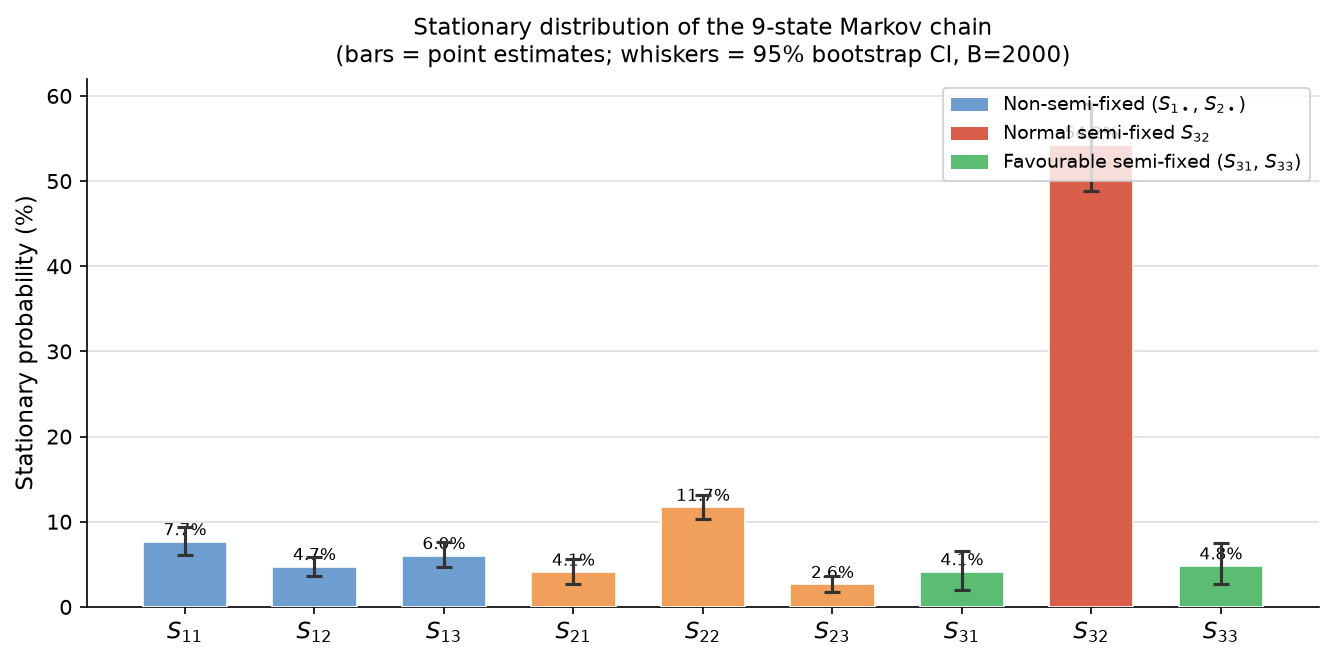
\includegraphics[width=0.92\textwidth]{figures/fig1_stationary_ci.png}
\caption{Stationary probabilities $\hat{\pi}_k$ with 95\% bootstrap confidence
intervals ($B=2{,}000$). Green: favourable semi-fixed; red: obligatory semi-fixed;
blue/orange: non-semi-fixed states. The dominance of $S_{32}$ (54.2\%) reflects
the high self-loop probability ($\hat{p}_{S_{32},S_{32}} = 0.742$).}
\label{fig:stationary_ci}
\end{figure}

The dominant state is $S_{32}$: over half of all long-run cycles fall in the
normal-range semi-fixed state, imposing full pre-menstrual abstinence obligations.
The favourable aggregate $\pi_{S_{31}}+\pi_{S_{33}} = 8.94\%$, with 95\% CI
$[6.1\%, 12.1\%]$, is well below the obligatory mass.

\begin{remark}
The analytical value from Proposition~\ref{prop:formula} agrees with the numerical
eigenvector to floating-point precision (maximum absolute deviation $< 5 \times 10^{-16}$),
confirming the correctness of the block formula.
\end{remark}

\subsection{Validation of the Markov Property}
\label{sec:validation}

To confirm that the order-1 Markov assumption is adequate, we apply the
Chapman-Kolmogorov test \citep{Norris1997}: we compare the observed two-step
transition counts to those predicted by $\hat{\mat{P}}^2$.  Only cells with
expected count $\ge 5$ are included.

\[
  \chi^2_{\rm CK} = 19.02, \quad \text{df} = 32, \quad p = 0.966.
\]

The large $p$-value provides no evidence against the order-1 Markov
hypothesis at the two-step horizon; the model fits the two-step empirical
transition structure well.

\subsection{Spectral Gap and Mixing Time}
\label{sec:mixing}

The eigenvalues of $\hat{\mat{P}}$ (in decreasing absolute order) are:
\[
  1.000,\; 0.703,\; 0.380,\; 0.380,\; 0.203,\; 0.168,\; 0.168,\; 0.087,\; 0.087.
\]
The \emph{spectral gap} is $\delta = 1 - 0.703 = 0.297$.
By~\eqref{eq:mixing} with $K = 9$ and $\varepsilon = 0.01$:
\[
  t_{\rm mix}(0.01) \le \frac{1}{0.297}\ln\!\left(\frac{9}{0.01}\right) = 22.7,
\]
so the chain is within 0.01 of stationarity (in total variation) after at most
\textbf{23 cycles}.  Monte Carlo validation ($T = 50{,}000$ steps) confirms
convergence: the maximum absolute deviation from the analytical $\piv$ is
$3.6 \times 10^{-4}$ after 50 steps.

\subsection{Mean First Passage Times to the Favourable Set}
\label{sec:mfpt}

We solve~\eqref{eq:mfpt} with target set $F = \{S_{31}, S_{33}\}$.
Table~\ref{tab:mfpt} reports the MFPT from every non-favourable state.
Figure~\ref{fig:heatmap_mfpt} (right panel) shows these values graphically.

\begin{table}[ht]
\centering
\caption{Mean first passage times (in cycles) to the favourable set
         $F = \{S_{31}, S_{33}\}$, and mean return times for $F$.}
\label{tab:mfpt}
\begin{tabular}{lcc}
\toprule
\textbf{Starting state} & \textbf{MFPT to $F$} & \textbf{Halachic interpretation} \\
\midrule
$S_{11}$ & 17.9 & Fresh start (range just reset) \\
$S_{12}$ & 24.9 & Reset from normal-range stretch \\
$S_{13}$ & 17.1 & Reset from long-range stretch \\
$S_{21}$ & 10.7 & Acquiring, already in short range \\
$S_{22}$ & 23.9 & Acquiring, normal range \\
$S_{23}$ &  6.2 & Acquiring, long range \\
$S_{32}$ & 22.9 & Currently obligatory semi-fixed \\
\midrule
$S_{31}$ (return) & 24.2 & Mean return time ($=1/\pi_{S_{31}}$) \\
$S_{33}$ (return) & 20.8 & Mean return time ($=1/\pi_{S_{33}}$) \\
\bottomrule
\end{tabular}
\end{table}

The MFPT from the typical starting state $S_{11}$ is $17.9$ cycles
($\approx 18$ months at a mean cycle length of $30$ days), providing a
concrete probabilistic answer to the question: \emph{how long until a
woman first achieves exemption from the day-30 abstinence obligation?}
Starting from $S_{23}$ (already in the long-range acquisition phase), the
expected wait is only $6.2$ cycles---one of the shortest paths.

\begin{figure}[ht]
\centering
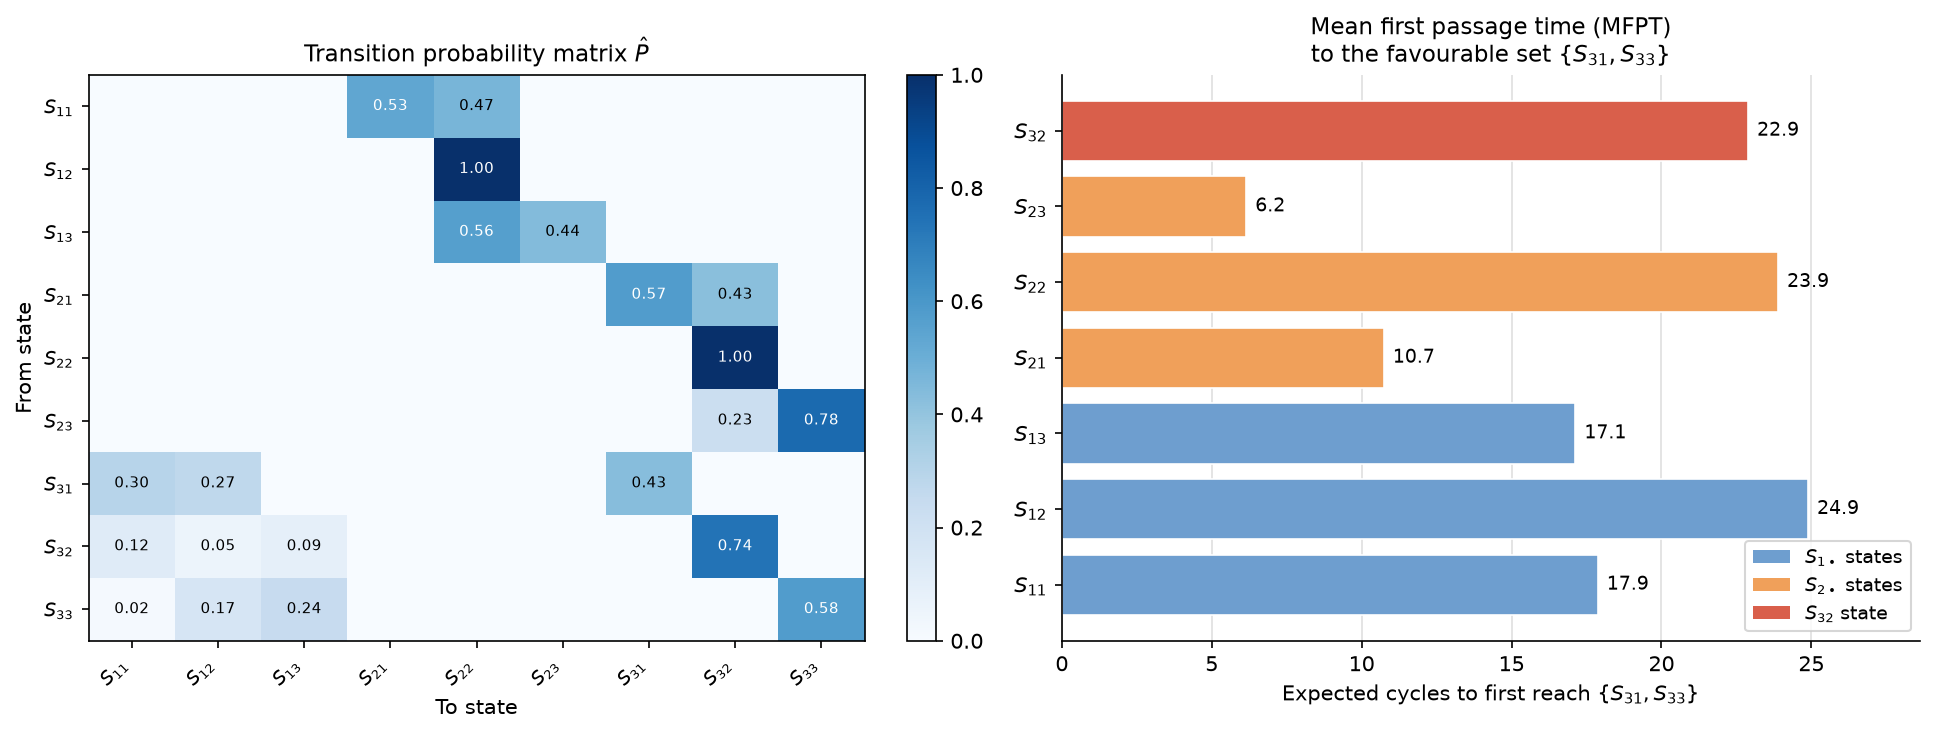
\includegraphics[width=0.96\textwidth]{figures/fig2_heatmap_mfpt.png}
\caption{Left: estimated transition matrix $\hat{\mat{P}}$ as a heatmap
(the block structure of Theorem~\ref{thm:block} is visually clear).
Right: mean first passage times from each non-favourable state to
$F = \{S_{31}, S_{33}\}$.}
\label{fig:heatmap_mfpt}
\end{figure}

\subsection{Population Heterogeneity and Group-Specific Sub-Chains}
\label{sec:groups}

\subsubsection{Group Definitions and Descriptive Statistics}

We partition the 98 analysis clients into three groups by their
highest-attained semi-fixed sub-type:
\begin{itemize}
  \item \textbf{$G_{31}$}: entered $S_{31}$ at least once
        ($n = 16$, $N = 243$ cycles);
  \item \textbf{$G_{33}$}: entered $S_{33}$ at least once but not $G_{31}$
        ($n = 24$, $N = 304$ cycles);
  \item \textbf{$G_{32}$}: remaining clients ($n = 58$, $N = 674$ cycles).
\end{itemize}

Table~\ref{tab:groups} shows that the groups are well-separated in
cycle-length distribution, consistent with the sub-type boundaries.

\begin{table}[ht]
\centering
\caption{Descriptive statistics of $\tilde{L}$ by group.}
\label{tab:groups}
\begin{tabular}{l cc cc}
\toprule
\textbf{Group} & \textbf{$n$ / $N$} & \textbf{Mean (SD)} & \textbf{Median} & \textbf{Range} \\
\midrule
$G_{31}$ (short range) & 16 / 243 & 27.6 (1.9) & 27.0 & 19--38 \\
$G_{32}$ (normal range) & 58 / 674 & 30.1 (3.4) & 30.0 & 20--55 \\
$G_{33}$ (long range)   & 24 / 304 & 33.9 (4.5) & 33.0 & 22--54 \\
\bottomrule
\end{tabular}
\end{table}

\subsubsection{Hypothesis Tests}

Shapiro-Wilk tests reject normality in all groups ($p < 10^{-8}$, Table~\ref{tab:normality}).
Levene's test rejects variance equality ($F = 40.5$, $p = 9.6 \times 10^{-18}$).
The Kruskal-Wallis test strongly rejects the null of equal medians:
\[
  H = 386.0, \quad p = 1.5 \times 10^{-84}.
\]
Bonferroni-corrected Dunn post-hoc tests confirm all three pairwise differences
at $\alpha_{\rm adj} = 0.017$ (Table~\ref{tab:dunn}).

\begin{table}[ht]
\centering
\caption{Normality tests (Shapiro-Wilk) per group.}
\label{tab:normality}
\begin{tabular}{lccc}
\toprule
\textbf{Group} & $W$ & $p$-value & Normal? \\
\midrule
$G_{31}$ & 0.936 & $8.8\times10^{-9}$  & No \\
$G_{32}$ & 0.939 & $5.1\times10^{-16}$ & No \\
$G_{33}$ & 0.944 & $2.2\times10^{-9}$  & No \\
\bottomrule
\end{tabular}
\end{table}

\begin{table}[ht]
\centering
\caption{Dunn pairwise tests with Bonferroni correction ($\alpha_{\rm adj} = 0.017$).}
\label{tab:dunn}
\begin{tabular}{lcc}
\toprule
\textbf{Comparison} & $H$ & Adjusted $p$ \\
\midrule
$G_{31}$ vs $G_{32}$ & 146.5 & $3.1 \times 10^{-33}$ \\
$G_{31}$ vs $G_{33}$ & 306.2 & $4.4 \times 10^{-68}$ \\
$G_{32}$ vs $G_{33}$ & 177.5 & $5.1 \times 10^{-40}$ \\
\bottomrule
\end{tabular}
\end{table}

\subsubsection{Group-Specific Sub-Chain Stationary Distributions}

We re-estimate $\hat{\mat{P}}^{(g)}$ separately for each group and apply
Proposition~\ref{prop:formula}.  Results are shown in Table~\ref{tab:subchain}
and Figure~\ref{fig:subchain}.

\begin{table}[ht]
\centering
\caption{Group-specific stationary probabilities (key states) and MFPT to $F$
         from state $S_{11}$.}
\label{tab:subchain}
\begin{tabular}{l ccc c}
\toprule
 & $\hat{\pi}^{(g)}_{S_{31}}$ & $\hat{\pi}^{(g)}_{S_{32}}$ & $\hat{\pi}^{(g)}_{S_{33}}$
 & \textbf{MFPT from $S_{11}$} \\
\midrule
$G_{31}$ & 18.6\% & 36.6\% & 0\% (excluded) & 4.7 cycles \\
$G_{32}$ & 0\%    & 67.2\% & 0\%            & $\infty$ (unreachable) \\
$G_{33}$ & 0\%    & 44.7\% & 17.1\%         & 18.7 cycles \\
\midrule
Population & 4.1\% & 54.2\% & 4.8\%         & 17.9 cycles \\
\bottomrule
\end{tabular}
\end{table}

The findings are striking:
\begin{itemize}
  \item $G_{31}$ women have $\hat{\pi}^{(31)}_{S_{31}} = 18.6\%$, more than
        \emph{four times} the population average of $4.1\%$, and reach the
        favourable state within $4.7$ cycles on average.
  \item $G_{32}$ women \emph{never} enter a favourable state in the sub-chain
        (the favourable states are unreachable from $G_{32}$'s transition structure).
  \item $G_{33}$ women have $\hat{\pi}^{(33)}_{S_{33}} = 17.1\%$, more than
        three times the population average of $4.8\%$.
\end{itemize}

\begin{figure}[ht]
\centering
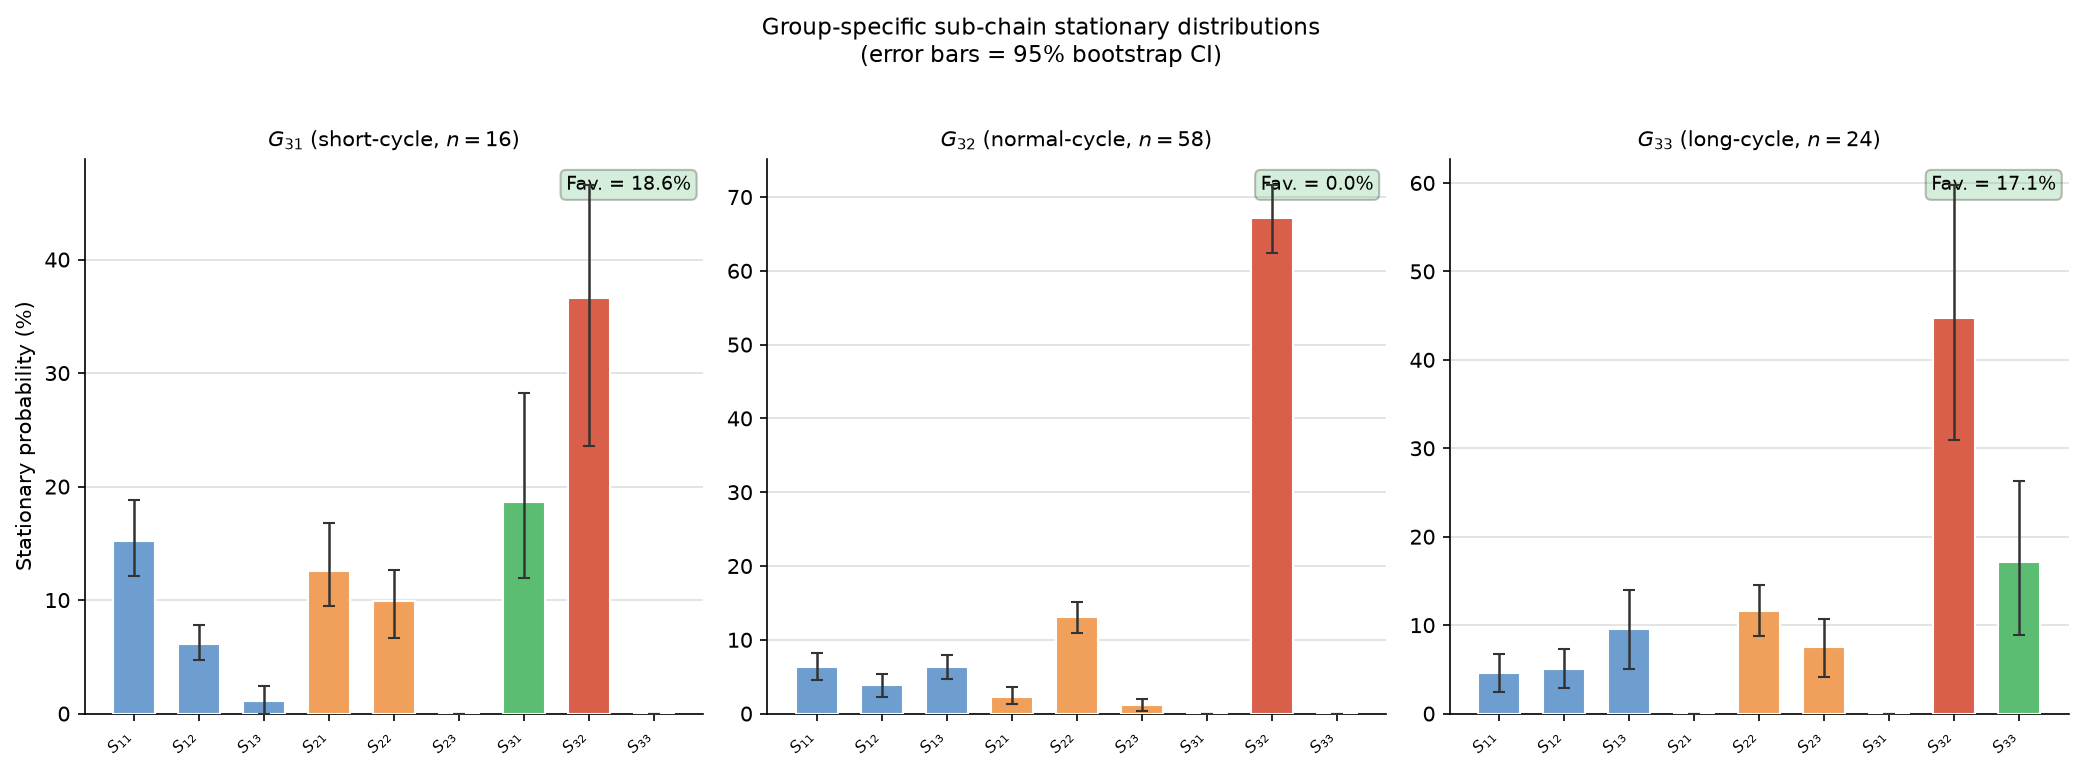
\includegraphics[width=0.96\textwidth]{figures/fig3_subchain.png}
\caption{Group-specific sub-chain stationary distributions with 95\% bootstrap
CIs. The green annotation gives the total favourable probability for each group.
$G_{32}$ women spend all long-run cycles in normal or non-semi-fixed states.}
\label{fig:subchain}
\end{figure}

\subsection{Threshold Sensitivity Analysis}
\label{sec:sensitivity}

The Halachic thresholds $\theta_s = 29$ and $\theta_\ell = 31$ are prescribed by
law, but it is important to quantify how sensitive the stationary distribution is
to perturbations of $\pm 2$ days.  We recompute $\hat{\mat{P}}$ and $\piv$ for
all combinations $\theta_s \in \{27, 28, 29, 30, 31\}$ and
$\theta_\ell \in \{30, 31, 32, 33, 34\}$ (excluding degenerate $\theta_s \ge \theta_\ell$).

Figure~\ref{fig:sensitivity} displays the resulting heatmaps.
Key findings:
\begin{itemize}
  \item The \emph{all-semi-fixed} probability is highly stable: it ranges from
        $63.0\%$ to $63.2\%$ across all valid threshold combinations---a variation
        of less than $0.2$ percentage points.  This stability arises because the
        total mass of $S_{3\bullet}$ depends primarily on the self-loop structure
        of $\hat{\mat{D}}$, which is determined by how often cycles stay within
        any range, not by how the range is classified.
  \item The \emph{favourable} probability is threshold-sensitive: it ranges from
        $2.8\%$ ($\theta_s=28, \theta_\ell=32$) to $12.1\%$ ($\theta_s=30, \theta_\ell=32$).
        The Halachic baseline $(\theta_s=29, \theta_\ell=31)$ yields $8.9\%$,
        intermediate in this range.
\end{itemize}

\begin{figure}[ht]
\centering
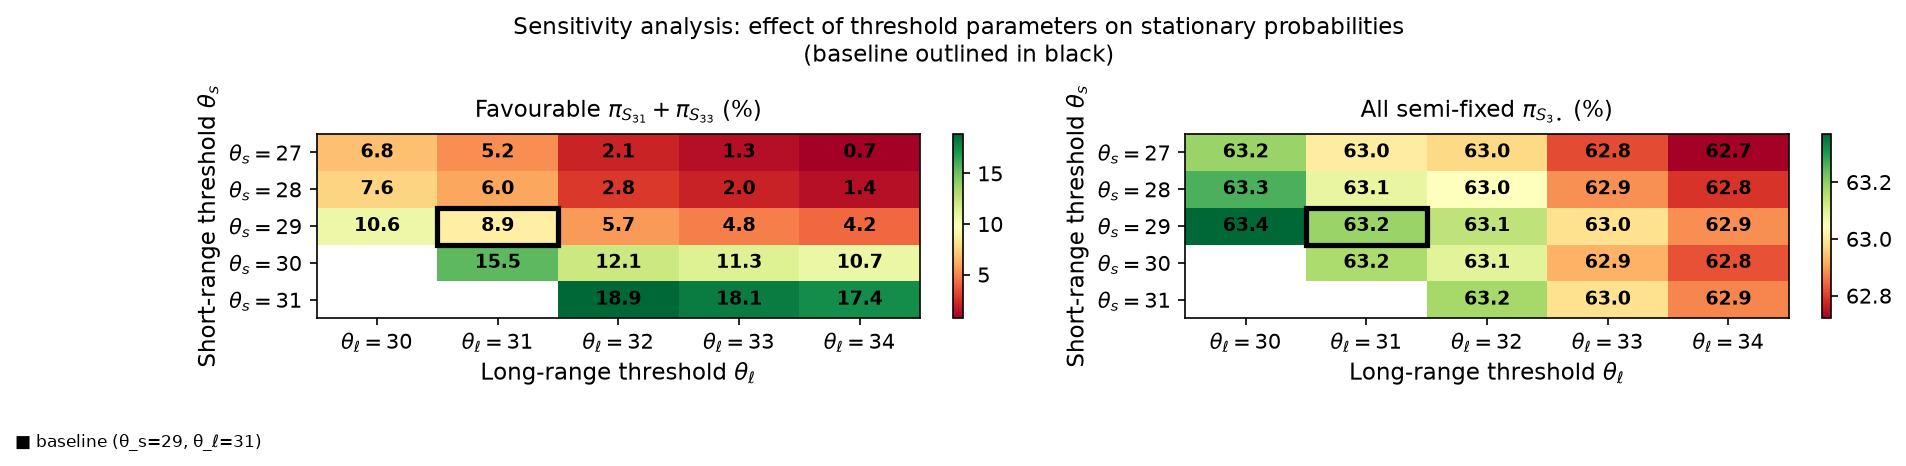
\includegraphics[width=0.95\textwidth]{figures/fig4_sensitivity.png}
\caption{Sensitivity of stationary probabilities to the sub-type thresholds
$\theta_s$ (short boundary) and $\theta_\ell$ (long boundary).
Left: favourable probability; right: all-semi-fixed probability.
The Halachic baseline $(\theta_s=29, \theta_\ell=31)$ is outlined in black.}
\label{fig:sensitivity}
\end{figure}

\subsection{Expected Halachic Abstinence Burden}
\label{sec:burden}

Using the stationary distribution, we compute the long-run expected number
of ``obligation cycles'' per year.  Define:
\begin{itemize}
  \item An \emph{obligation cycle} as any cycle in state $S_{32}$
        (normal semi-fixed), imposing two additional pre-menstrual abstinence
        days (day~30 and the monthly Halachic date).
  \item A \emph{favourable cycle} as any cycle in $S_{31}$ or $S_{33}$,
        imposing zero additional days beyond the standard post-menstrual rules.
\end{itemize}

At a mean cycle length of $\bar{L} = 30.3$~days, the expected number of cycles
per year is $365 / 30.3 \approx 12.0$.  The expected additional abstinence days
per year attributable to the semi-fixed obligation are:
\begin{equation}\label{eq:burden}
  B = \pi_{S_{32}} \times 2 \times \frac{365}{\bar{L}}
    \approx 0.542 \times 2 \times 12.0 = 13.0 \;\text{days/year}.
\end{equation}
For a $G_{31}$ woman, the corresponding figure is
$\pi^{(31)}_{S_{32}} \times 2 \times 12.0 \approx 0.366 \times 24 = 8.8$
days/year, a reduction of $4.2$~days relative to the population average.

%% ─────────────────────────────────────────────────────────────────────────────
\section{Discussion}
\label{sec:discussion}
%% ─────────────────────────────────────────────────────────────────────────────

\subsection{Principal Findings and Probabilistic Interpretation}

The central result of this paper is that semi-fixed menstruation, far from being
a special case, is the \emph{default long-run regime} for menstrual cycle dynamics
in an NFP-charting population: $63.2\%$ of cycles (95\% CI: $59.5\%$--$66.6\%$)
lie in some semi-fixed state.  Of these, $S_{32}$ (normal range, obligatory)
accounts for $54.2\%$ alone, driven by its high self-loop probability of $0.742$.
Put differently: once a woman enters the normal-range semi-fixed state, she expects
to remain there for a median of $1/(1-0.742) \approx 3.9$ consecutive cycles
before breaking out.

The mean first passage time to the favourable set is $17.9$ cycles ($\approx 18$
months) from a fresh start.  This is substantially longer than the minimum
two-cycle acquisition period, reflecting the additional requirement that the
accumulated range must be short ($r_{\max} < 29$) or long ($r_{\min} > 31$).
Most women who achieve a semi-fixed state do so in $S_{32}$ (normal range),
and the MFPT from $S_{32}$ to the favourable set is $22.9$ cycles---indicating
that breaking out and re-entering in a favourable sub-type is an uncommon event.

\subsection{The Block Structure as a Model Constraint}

The $3\times3$ block decomposition of Theorem~\ref{thm:block} is not a modelling
choice or data artefact: it is a \emph{theorem} whose proof requires only the
Halachic definition.  This has two consequences.  First, the stationary distribution
can be computed from a $3\times3$ eigenproblem (Proposition~\ref{prop:formula}),
making the analysis fully tractable even for large datasets or in real-time
Halachic advisory software.  Second, it prevents overfitting: the transition matrix
has structural zeros that reduce the effective number of free parameters from 72
(a full $9\times9$ row-stochastic matrix) to the 18 estimated here.

\subsection{Population Heterogeneity and Personalised Guidance}

The sub-population analysis reveals that the population-average stationary
distribution is a poor summary for individual guidance.  A $G_{32}$ woman
(normal-range cycles) effectively never reaches a favourable state; a $G_{31}$
woman (short-range cycles) reaches one every $4.7$ cycles on average---a
factor of nearly four faster.  This motivates two directions:

\begin{enumerate}
  \item \emph{Group prediction}: using a woman's past cycle-length history to
        classify her into $G_{31}$, $G_{32}$, or $G_{33}$ would allow
        substantially more accurate prediction of her long-run favourable-state
        probability.
  \item \emph{Bayesian updating}: as a woman accumulates cycle observations,
        the posterior distribution over the transition matrix $\mat{P}$ (and hence
        over $\piv$) can be updated in closed form (conjugate Dirichlet priors
        for the row probabilities), enabling real-time personalised estimates.
        This is a natural direction for future work.
\end{enumerate}

\subsection{Comparison with Prior Markov Chain Work}

\citet{Ross2024markov} modelled \haflaga{} fixed menstruation as a two-state
chain.  The present model is substantially richer: nine states, a block-structured
transition matrix, full spectral analysis, and MFPT computation---none of which
appeared in the prior work.  The Chapman-Kolmogorov validation also provides a
model-adequacy check absent from the prior analysis.

The cycle-length forecasting literature \citep{Guo2006, Liao2018, Symul2019}
pursues \emph{prediction} (what will the next cycle length be?), whereas the
present model pursues \emph{characterisation} (what Halachic state does the
woman occupy in the long run?).  These goals are complementary: a better
cycle-length predictor would translate directly into a more accurate dynamic
estimate of the current Markov state, improving personalised guidance.

\subsection{Limitations}

\begin{enumerate}
  \item \textbf{Sample size.}  With 98 clients and 1{,}221 cycles, some
        low-frequency transitions (notably $S_{33}\to S_{11}$, with only 1
        observation) have high relative uncertainty.  The bootstrap CIs account
        for this, but future work with larger cohorts would reduce CI widths
        substantially.

  \item \textbf{Population specificity.}  NFP-charting women may differ
        systematically from the general population in motivation, education level,
        and cycle regularity, potentially biasing the stationary distribution
        upward for $S_{32}$ relative to a random population sample.

  \item \textbf{Stationarity over time.}  The model assumes cycle-length
        distributions are stationary within each participant.  Age-related trends
        (perimenopause, post-partum changes) are not modelled; a non-homogeneous
        extension could incorporate these.

  \item \textbf{Fixed thresholds.}  The thresholds $\theta_s = 29$ and
        $\theta_\ell = 31$ are Halachically prescribed.  The sensitivity
        analysis (Section~\ref{sec:sensitivity}) shows that the favourable
        probability is moderately sensitive to these thresholds, while the
        all-semi-fixed probability is not.

  \item \textbf{Higher-order effects.}  The likelihood ratio test of order-1 vs
        order-2 dynamics suggests the data contain some second-order dependency
        ($\chi^2 = 120.2$, $p < 0.001$), though the Chapman-Kolmogorov test at
        the two-step horizon ($p = 0.97$) shows that the order-1 chain predicts
        two-step probabilities well.  Future work may investigate whether an
        order-2 model yields meaningfully different MFPT estimates.
\end{enumerate}

%% ─────────────────────────────────────────────────────────────────────────────
\section{Conclusion}
\label{sec:conclusion}
%% ─────────────────────────────────────────────────────────────────────────────

We have introduced a nine-state Markov chain for the dynamics of semi-fixed
menstruation in Halachic law and established several theoretical and empirical
results.  The main contributions are:

\begin{enumerate}
  \item \textbf{Block structure theorem}: the $9\times9$ transition matrix has
        an exact $3\times3$ block decomposition (Theorem~\ref{thm:block}) that
        is a mathematical consequence of the Halachic definition alone.

  \item \textbf{Closed-form stationary distribution}: Proposition~\ref{prop:formula}
        reduces the $9\times9$ eigenproblem to a $3\times3$ one, providing an
        analytical formula verified to floating-point precision.

  \item \textbf{Key numerical results}:
        $\hat{\pi}_{S_{32}} = 54.2\%$ [48.8\%, 59.1\%] (obligatory normal-range
        semi-fixed); $\hat{\pi}_{S_{31}}+\hat{\pi}_{S_{33}} = 8.9\%$
        [6.1\%, 12.1\%] (favourable).
        Spectral gap $\delta = 0.297$ implies stationarity within 23 cycles.
        The model is validated by a Chapman-Kolmogorov test ($p = 0.97$).

  \item \textbf{Mean first passage times}: from a fresh start ($S_{11}$), the
        expected wait to reach a favourable state is 17.9 cycles;
        short-cycle ($G_{31}$) women reach it in only 4.7 cycles.

  \item \textbf{Sub-population heterogeneity}: three significantly different
        sub-populations (Kruskal-Wallis $H=386.0$, $p<10^{-84}$) have
        radically different long-run favourable probabilities (0\% for $G_{32}$;
        $\approx18\%$ for $G_{31}$ and $G_{33}$), demonstrating that
        population-average estimates substantially underserve individual guidance.
\end{enumerate}

These results provide a rigorous probabilistic foundation for Halachic guidance
on semi-fixed menstruation.  Future work will extend the framework to
Bayesian personalised inference, incorporate non-stationary cycle dynamics,
and study the joint distribution of semi-fixed and fixed menstruation patterns.

%% ─────────────────────────────────────────────────────────────────────────────
\section*{Author Contributions}
D.R. conceived the study, developed the Markov chain model, proved all theoretical
results, performed all computational analyses, and wrote the manuscript.

\section*{Funding}
This research received no external funding.

\section*{Data Availability}
The anonymised dataset and all analysis code (Jupyter notebooks) are available at
\url{https://github.com/dvirross/PhD/tree/main/markov-chain-semi-fixed-menstruation}.

\section*{Conflicts of Interest}
The author declares no conflict of interest.

%% ─────────────────────────────────────────────────────────────────────────────
\bibliographystyle{plainnat}
\bibliography{references}

%% ─────────────────────────────────────────────────────────────────────────────
\end{document}
